\begin{highlightblock}[Adder]
Write an entity and architecture for the system described in Figure \ref{fig:add}. This entity has two inputs (\vhdl{operand_a_i} and \vhdl{operand_b_i}) and one output. The inputs and outputs of this entity are no single bits but bit vectors (use \vhdl{std_ulogic} vectors). The output \vhdl{result_o} should be calculated as the arithmetical sum of the two inputs. The bit width of the inputs (both should have the same bit width) should be defined by a generic \vhdl{BITWIDTH}. The output bit width should also be defined via this generic (but is of course not equal to this generic...).
\begin{center}
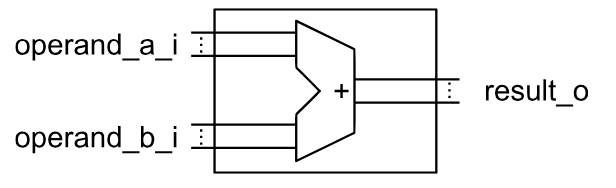
\includegraphics[width=0.5\linewidth]{images/adder.png}

Figure \refstepcounter{figure}\arabic{figure}: Adder\label{fig:add}
\end{center}

\textbf{To-Do-List}

\begin{itemize}
\item Write the entity and the architecture of the system in VHDL. Use one .vhd file for the entity and one .vhd file for the architecture. Describe: how you have defined the output bit width? Give the reasons (few sentences) for your definition.
\item Write a testbench in VHDL (extra file). Test the system and hand in screenshots showing the output of the waveform window. Do two tests with different bit widths ($\leq$ 3 bits). Think of useful test cases (at least 5 different ones for every bit width). In a few sentences summarize the reasons why you have chosen these test cases. In addition do one test where you add two times the maximum value of the inputs. Discuss the result of the simulation in a few sentences. Do you need additional output bits?
\end{itemize}

\end{highlightblock}